\chapter{3D model assessment}

    \section{Contact-assisted 3D modelling}

    This appendix describes the algorithm used to reconstruct
    proteins in three dimensions. Like GDFuzz3D~\cite{pietal2015gdfuzz3d},
    it uses graph distances to convert predicted contact maps
    in order to approximate distance maps. However, the proposed method is template-free
    and does not make use of MODELLER~\cite{modeller} as in GDFuzz3D.

    \subsection{Graph distances}

        Let's use the graph representation of contact maps as in section \ref{pcn}
        about Protein Contact Networks.
        The graph distance between two residues is defined as the length of
        the shortest path between them.
        Predicted contact maps are converted to binary adjacency matrices
        by keeping only the $4.5\,L$ top predicted contacts.

    \subsection{Approximate Euclidean distances}

        As explained in \cite{pietal2015gdfuzz3d}, there is a linear relationship
        between graph distances and real euclidean distances.
        Let $GD_{i,j}$ be the graph distance between residues $i$ and $j$. Then
        the euclidean distance $\dis(\mathbf{x_i},\mathbf{x_j})$ between the corresponding
        points $x_i$ and $x_j$ is approximated by:

        \begin{align}
            \dis(\mathbf{x_i},\mathbf{x_j}) = 5.72 \times GD_{i,j}
        \end{align}

        It must be noted that the error on the euclidean distance also increases
        with graph distance. For all residue pairs for which no tractable information
        is available and no protein template is available,
        this estimated distance remains the best estimator.

    \subsection{Gaussian restraints}

        Each residue pair may be associated to at most one Gaussian restraint.
        A Gaussian restraint is defined by its mean and standard deviation,
        computed empirically over a set of distances with specific properties
        like graph distances, sequence separation or secondary structure.

        As an example, residue pairs with a graph distance of one (residues are
        in contact) and a sequence separation of one have an average distance equal
        to the $C_{\alpha}-C_{\beta}$ distance (3.82 \AA{}), and a standard deviation
        equal to 0.35 \AA{}.

        \begin{table}[H]
            \centering
            \begin{tabular}{|l|c|c|c|}
                \hline
                Restraint type & Seq. sep. & Mean & Standard deviation \\
                \hline
                \hline
                Repulsion     & $\ge$ 6 & 20.00 & 120.00 \\
                Interior      & - & 5.00 & 10.00 \\
                Adjacent      & 1 & 3.81 & 0.1  \\
                Next adjacent & 2 & 5.20 & 0.55 \\
                Next adjacent & 3 & 7.00 & 0.71 \\
                Intra-alpha   & 1 & 3.82 & 0.35 \\
                Intra-alpha   & 2 & 5.50 & 0.52 \\
                Intra-alpha   & 3 & 5.33 & 0.93 \\
                Intra-alpha   & 4 & 6.42 & 1.04 \\
                Intra-beta    & 1 & 3.80 & 0.28 \\
                Intra-beta    & 2 & 6.66 & 0.30 \\
                Alpha/beta    & $\ge$ 4 & 6.05 & 0.95 \\
                Helix/coil    & $\ge$ 4 & 6.60 & 0.92 \\
                All & $\ge$ 4 & 5.72 $\times$ GD & 1.34 $\times$ GD \\
                \hline
            \end{tabular}
            \captionof{table}{Gaussian restraints present in the 3D model}
            \label{restraints}
        \end{table}

        The set of points $X$ that best satisfies Gaussian restraints is simply
        obtained by log-likelihood maximization:
        \begin{align}
            \hat{X} & = \argmax_{X} \sum\limits_{i < j ,\, (\mu_{i,j}, \sigma_{i,j}) \in R}
                \Bigg(\frac{\delta(x_i, x_j) - \mu_{i,j}}{\sigma_{i,j}}\Bigg)^2
        \end{align}

        where $R$ is the set of parameters of the Gaussian restraints. This notation is used
        because all residue pairs may not be restrained.

        \todo{\cite{reese1996distance}}

    \subsection{Evolutionary algorithm}

        Gaussian log-likelihood is maximized by a vanilla genetic algorithm.
        The initial population is obtained by adding random noise to the coordinates
        predicted by the multidimensional scaling algorithm.
        Parent selection is done by creating two random partitions from current population
        and keeping the individuals that maximize log-likelihood in each one.
        A new individual is then created by taking each point from either the first
        or the second parent, randomly. Mutation is simulated by adding Gaussian noise
        to each point with a 50\% chance.
        Finally, the individual with lowest log-likelihood is replaced by the
        newly created individual.

        The set of hyper-parameters is composed of:
        \begin{itemize}
            \item Population size (default value is 2000)
            \item Partition size (default value is 50)
            \item Maximum number of iterations (default value is 200000)
            \item Standard deviation of mutation noise (default value is 10)
        \end{itemize}

    \section{Evaluation metrics}

    \begin{align}
        \text{TM-score}(X^{(target)}, X^{(aligned)}) = \max_P \Bigg[ \frac{1}{L} \sum\limits_{i=1}^L
            \frac{1}{1 + \Big(\frac{\delta(x_i^{(target)}, x_i^{(aligned)})}{\delta_0}\Big)^2} \Bigg]
    \end{align}

    where $\delta_0 = 1.24 \sqrt[3]{L - 15} - 1.8$, and $P$ is a projection that preserves

    The best alignment in 3D is found by determining the projection of $X^{(aligned)}$ that
    either maximizes the TM-score or minimizes the RMSD.
    Such a projection has 9 parameters:
    \begin{itemize}
        \item 3 boolean parameters that indicate whether to swap coordinates along
        the X, Y and Z dimensions, respectively.
        \item 3 real-valued parameters for translating coordinates along the X, Y and Z
        dimensions, respectively.
        \item 3 angles that parametrize the rotation matrices around the X, Y and Z axes,
        respectively.
    \end{itemize}

    \begin{align*}
        P(x) & = R^X_{\phi} R^Y_{\psi} R^Z_{\theta} x + b \\
        & =
        \begin{pmatrix}
        1 & 0 & 0 \\
        0 & \cos{\phi} & -\sin{\phi} \\
        0 & \sin{\phi} & \cos{\phi}
        \end{pmatrix}
        \begin{pmatrix}
        \cos{\psi} & 0 & \sin{\psi} \\
        0 & 1 & 0 \\
        -\sin{\psi} & 0 & \cos{\psi}
        \end{pmatrix}
        \begin{pmatrix}
        \cos{\theta} & -\sin{\theta} & 0 \\
        \sin{\theta} & \cos{\theta} & 0 \\
        0 & 0 & 1
        \end{pmatrix}
        x +
        \begin{pmatrix}
        b^X \\
        b^Y \\
        b^Z
        \end{pmatrix}
    \end{align*}

\section{Evaluation of GDE-GaussFold}

    \begin{figure}[H]
      \begin{center}
        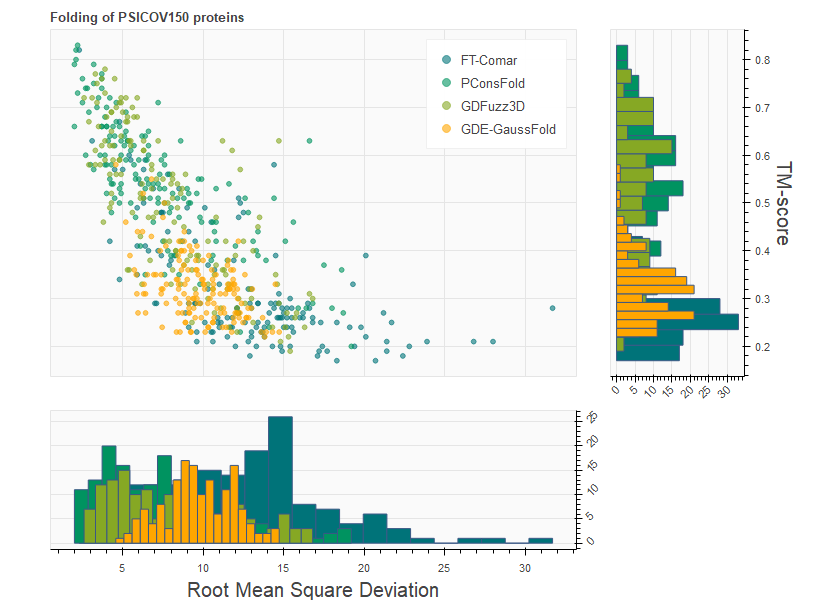
\includegraphics[width=\textwidth, keepaspectratio]{imgs/gde.png}
         \caption{TM-scores and RMSD of different folding methods including
         GDE-GaussFold, with density functions on the sides.}
        \label{gde_results}
      \end{center}
    \end{figure}

